\documentclass[a4 paper]{article}

\usepackage[inner=2.0cm,outer=2.0cm,top=2.5cm,bottom=2.5cm]{geometry}
\usepackage{setspace}
\usepackage[rgb]{xcolor}
\usepackage{verbatim}
\usepackage{subcaption}
\usepackage{amsgen,amsmath,amstext,amsbsy,amsopn,tikz,amssymb,tkz-linknodes}
\usepackage{fancyhdr}
\usepackage[colorlinks=true, urlcolor=blue,  linkcolor=blue, citecolor=blue]{hyperref}
\usepackage[colorinlistoftodos]{todonotes}
\usepackage{rotating}
\usepackage{graphicx}
\usepackage{minted}

\allowdisplaybreaks
\DeclareMathOperator*{\argmin}{\arg\min} 
\DeclareMathOperator*{\argmax}{\arg\max} 

\hypersetup{%
pdfauthor={Vineeth S},%
pdftitle={Homework},%
pdfkeywords={Tikz,latex,bootstrap,uncertaintes},%
pdfcreator={PDFLaTeX},%
pdfproducer={PDFLaTeX},%
}

\usepackage{booktabs}
\newcommand{\ra}[1]{\renewcommand{\arraystretch}{#1}}

\newtheorem{thm}{Theorem}[section]
\newtheorem{prop}[thm]{Proposition}
\newtheorem{lem}[thm]{Lemma}
\newtheorem{cor}[thm]{Corollary}
\newtheorem{defn}[thm]{Definition}
\newtheorem{rem}[thm]{Remark}
\numberwithin{equation}{section}

\newcommand{\homework}[6]{
   \pagestyle{myheadings}
   \thispagestyle{plain}
   \newpage
   \setcounter{page}{1}
   \noindent
   \begin{center}
   \framebox{
      \vbox{\vspace{2mm}
    \hbox to 6.28in { {\bf E1 244:~Detection and Estimation Theory\hfill {\small (#2)}} }
       \vspace{6mm}
       \hbox to 6.28in { {\Large \hfill #1  \hfill} }
       \vspace{6mm}
       \hbox to 6.28in { {\it Instructor: {\rm #3} \hfill Name: {\rm #5}, SR No.: {\rm #6}} }
       %\hbox to 6.28in { {\it TA: #4  \hfill #6}}
      \vspace{2mm}}
   }
   \end{center}
   \markboth{#5 -- #1}{#5 -- #1}
   \vspace*{4mm}
}

\newcommand{\problem}[2]{~\\\fbox{\textbf{PART #1}}\hfill \newline\newline}
\newcommand{\subproblem}[1]{~\newline\textbf{#1}}
\newcommand{\D}{\mathcal{D}}
\newcommand{\Hy}{\mathcal{H}}
\newcommand{\VS}{\textrm{VS}}
\newcommand{\solution}{~\newline\textbf{\textit{(Solution)}} }

\newcommand{\bbF}{\mathbb{F}}
\newcommand{\bbX}{\mathbb{X}}
\newcommand{\bI}{\mathbf{I}}
\newcommand{\bX}{\mathbf{X}}
\newcommand{\bY}{\mathbf{Y}}
\newcommand{\bepsilon}{\boldsymbol{\epsilon}}
\newcommand{\balpha}{\boldsymbol{\alpha}}
\newcommand{\bbeta}{\boldsymbol{\beta}}
\newcommand{\0}{\mathbf{0}}
\linespread{1.5}


\begin{document}

\setlength{\abovedisplayskip}{3pt}
\setlength{\belowdisplayskip}{3pt}

\homework{Assignment \#1}{Due: 02/03/20}{Sundeep Chepuri}{}{Vineeth S}{16543}

\problem{A: Problem 1 Cramer-Rao Lower Bound (CRLB)}{}{}
\solution From the range difference equations we have,
\\ \centerline{$ r_{ij} = d_{i} - d_{j} + n_{ij} $}
\\ \centerline{$ n_{ij} = w_{i} - w_{j} $}

We will use a set of non redundant range equations,
\\ \centerline{$ r_{12} = d_{1} - d_{2} + n_{12} $}
\\ \centerline{$ r_{23} = d_{2} - d_{3} + n_{23} $}
\\ \centerline{$ r_{34} = d_{3} - d_{4} + n_{34} $}

Concisely in vector notation we can write as,
\[
\begin{bmatrix}
r_{12} \\ r_{23} \\ r_{34}
\end{bmatrix}
=
\begin{bmatrix}
d_{1} - d_{2} \\ d_{2}-d_{3} \\ d_{3}-d_{4}
\end{bmatrix}
+
\begin{bmatrix}
n_{12} \\ n_{23} \\ n_{34}
\end{bmatrix}
\]

\centerline{$ \mathbf{\underline{r}} = \mathbf{\underline{h}(\mathbf{\underline{x}})} + \mathbf{\underline{n}} $}
\centerline{$ \mathbf{\underline{r}} \sim \mathcal{N}(\mathbf{\underline{h}(\mathbf{\underline{x}})}, \mathbf{\Sigma_{n}})$}
where $\mathbf{\Sigma_{n}}$ is the noise covariance matrix, given by,
\[
\mathbf{\underline{n}} = 
\begin{bmatrix}
n_{12} \\ n_{23} \\ n_{34}
\end{bmatrix}
=
\begin{bmatrix}
1 & -1 & 0 & 0 \\ 0 & 1 & -1 & 0 \\ 0 & 0& 1 & -1 & 
\end{bmatrix}
\begin{bmatrix}
w_{1} \\ w_{2} \\ w_{3} \\ w_{4}
\end{bmatrix}
\]

\begin{align*}
\mathbf{\underline{n}} &= \mathbf{A}\mathbf{\underline{w}}
\\ \mathbf{\Sigma_{n}} &= E[\mathbf{\underline{n}}\mathbf{\underline{n}}^{T}]
\\ &=  E[\mathbf{A}\mathbf{\underline{w}}\mathbf{\underline{w}}^{T}\mathbf{A}]
\\ &= \mathbf{A}E[\mathbf{\underline{w}}\mathbf{\underline{w}}^{T}]\mathbf{A}^{T}
\\ &= \mathbf{A}\Sigma_{w}\mathbf{A}^{T}
\end{align*}

With this we can write the likelihood and log-likelihood functions as,
\begin{align*}
P(\mathbf{\underline{r}}; \mathbf{\underline{x}}) &= \frac{1}{(2\pi)^{3/2}|\sum_{n}|^{1/2}}exp(-\frac{1}{2}(\mathbf{\underline{r}}-\mathbf{\underline{h}(\mathbf{\underline{x}})})^{T}\Sigma_{n}^{-1}(\mathbf{\underline{r}}-\mathbf{\underline{h}(\mathbf{\underline{x}})}))
\\ ln P(\mathbf{\underline{r}}; \mathbf{\underline{x}}) &=  K -\frac{1}{2}(\mathbf{\underline{r}}-\mathbf{\underline{h}(\mathbf{\underline{x}})})^{T}\mathbf{\Sigma_{n}^{-1}}(\mathbf{\underline{r}}-\mathbf{\underline{h}(\mathbf{\underline{x}})})
\\ &= K - \frac{1}{2} \sum_{i =1}^{3}\sum_{j=1}^{3}(r_{i} - h_{i}(\mathbf{\underline{x})})[\mathbf{\Sigma_{n}^{-1}}]_{ij}(r_{j} - h_{j}(\mathbf{\underline{x}}))
\\ \frac{\partial}{\partial\mathbf{\underline{x}}}ln P(\mathbf{\underline{r}}; \mathbf{\underline{x}}) &= \frac{1}{2}\sum_{i =1}^{3}\sum_{j=1}^{3} [\mathbf{\Sigma_{n}^{-1}}]_{ij}(r_{i} - h_{i}(\mathbf{\underline{x}}))\frac{\partial h_{j}(\mathbf{\underline{x}})}{\mathbf{\partial\underline{x}}} + \frac{\partial h_{i}(\mathbf{\underline{x}})}{\mathbf{\partial\underline{x}}}(r_{j} - h_{j}(\mathbf{\underline{x}}))
\end{align*}

We can find the elements of the Fischer Information Matrix one element at a time,
\begin{align*}
\frac{\partial^{2}}{\partial x^{2}}ln P(\mathbf{\underline{r}}; \mathbf{\underline{x}})  &= \frac{1}{2}\sum_{i =1}^{3}\sum_{j=1}^{3} [\mathbf{\Sigma_{n}^{-1}}]_{ij} ((r_{i} - h_{i}(\mathbf{\underline{x}))}\frac{\partial^{2} h_{j}(\mathbf{\underline{x}})}{\partial x^{2}}-\frac{\partial h_{i}(\mathbf{\underline{x}})}{\partial x}\frac{\partial h_{j}(\mathbf{\underline{x}})}{\partial x} + (r_{j} - h_{j}(\mathbf{\underline{x}))}\frac{\partial^{2} h_{i}(\mathbf{\underline{x}})}{\partial x^{2}}-\frac{\partial h_{j}(\mathbf{\underline{x}})}{\partial x}\frac{\partial h_{i}(\mathbf{\underline{x}})}{\partial x})
\end{align*}

\vspace{-3.5em}

\begin{align*}
\\ [\mathbf{I(\mathbf{\underline{x}})}]_{11} &= -E[\frac{\partial^{2}}{\partial x^{2}}ln P(\mathbf{\underline{r}}; \mathbf{\underline{x}})]
\\ &= \sum_{i =1}^{3}\sum_{j=1}^{3} [\mathbf{\Sigma_{n}^{-1}}]_{ij}\frac{\partial h_{i}(\mathbf{\underline{x}})}{\partial x}\frac{\partial h_{j}(\mathbf{\underline{x}})}{\partial x}
\\ &= \frac{\partial \mathbf{\underline{h}}(\mathbf{\underline{x}})}{\partial x}^{T} \mathbf{\Sigma_{n}^{-1}} \frac{\partial \mathbf{\underline{h}(\mathbf{\underline{x}})}}{\partial x}
\\ [\mathbf{I(\mathbf{\underline{x}})}]_{12} &= -E[\frac{\partial^{2}}{\partial x \partial y}ln P(\mathbf{\underline{r}}; \mathbf{\underline{x}})]
\\ &= \sum_{i =1}^{3}\sum_{j=1}^{3} [\mathbf{\Sigma_{n}^{-1}}]_{ij}\frac{\partial h_{i}(\mathbf{\underline{x}})}{\partial x}\frac{\partial h_{j}(\mathbf{\underline{x}})}{\partial y}
\\ &= \frac{\partial \mathbf{\underline{h}}(\mathbf{\underline{x}})}{\partial x}^{T} \mathbf{\Sigma_{n}^{-1}} \frac{\partial \mathbf{\underline{h}(\mathbf{\underline{x}})}}{\partial y}
\\ [\mathbf{I(\mathbf{\underline{x}})}]_{21} &= -E[\frac{\partial^{2}}{\partial y \partial x}ln P(\mathbf{\underline{r}}; \mathbf{\underline{x}})]
\\ &= \sum_{i =1}^{3}\sum_{j=1}^{3} [\mathbf{\Sigma_{n}^{-1}}]_{ij}\frac{\partial h_{i}(\mathbf{\underline{x}})}{\partial y}\frac{\partial h_{j}(\mathbf{\underline{x}})}{\partial x}
\\ &= \frac{\partial \mathbf{\underline{h}}(\mathbf{\underline{x}})}{\partial y}^{T} \mathbf{\Sigma_{n}^{-1}} \frac{\partial \mathbf{\underline{h}(\mathbf{\underline{x}})}}{\partial x}
\\ [\mathbf{I(\mathbf{\underline{x}})}]_{22} &= -E[\frac{\partial^{2}}{\partial y \partial y}ln P(\mathbf{\underline{r}}; \mathbf{\underline{x}})]
\\ &= \sum_{i =1}^{3}\sum_{j=1}^{3} [\mathbf{\Sigma_{n}^{-1}}]_{ij}\frac{\partial h_{i}(\mathbf{\underline{x}})}{\partial y}\frac{\partial h_{j}(\mathbf{\underline{x}})}{\partial y}
\\ &= \frac{\partial \mathbf{\underline{h}}(\mathbf{\underline{x}})}{\partial y}^{T} \mathbf{\Sigma_{n}^{-1}} \frac{\partial \mathbf{\underline{h}(\mathbf{\underline{x}})}}{\partial y}
\end{align*}

where,
\[
\frac{\partial \mathbf{\underline{h}(\mathbf{\underline{x}})}}{\partial y} 
= 
\begin{bmatrix}
\frac{\partial h_{1}(\mathbf{\underline{x}})}{\partial x} & \frac{\partial h_{2}(\mathbf{\underline{x}})}{\partial x} & \frac{\partial h_{3}(\mathbf{\underline{x}})}{\partial x}
\end{bmatrix}
\]

\begin{align*}
\frac{\partial h_{i}(\mathbf{\underline{x}})}{\partial x} &= \frac{\partial}{\partial x} (d_{i} - d_{i+1})
\\ &= \frac{\partial}{\partial x}(||\mathbf{x}-\mathbf{x}_{i}||_{2} - ||\mathbf{x}-\mathbf{x}_{i+1}||_{2} )
\\ &= \frac{x- x_{i}}{||\mathbf{x}-\mathbf{x}_{i}||_{2}} - \frac{x- x_{i+1}}{||\mathbf{x}-\mathbf{x}_{i+1}||_{2}}
\\ &= \frac{x- x_{i}}{d_{i}} - \frac{x- x_{i+1}}{d_{i+1}}
\end{align*}

\newpage
Given an $\mathbf{\underline{x}}$, we can find the elements of Fischer Information Matrix and invert it to get the CRLB.
\\ \centerline{$ \mathbf{C}_{\mathbf{\hat{\underline{x}}}} \geq [\mathbf{I^{-1}(\mathbf{\underline{x}})}] $}
\\ \centerline{$ Var[{\hat{x}}] \geq [\mathbf{I^{-1}(\mathbf{\underline{x}})}]_{11} $}
\\ \centerline{$ Var[{\hat{y}}] \geq [\mathbf{I^{-1}(\mathbf{\underline{x}})}]_{22} $}






\newpage
\problem{A: Problem 2 Maximum Likelihood Estimator (MLE)}{}
\solution We want obtain the maximum likelihood estimator (MLE) for $\mathbf{\underline{x}}$. The estimator that aximizes likelihood function also maximizes log-likelihood, since log function is a monotonically increasing function.
\\ We have our likelihood and log-likelihood functions from Problem 1 as,
\begin{align*}
P(\mathbf{\underline{r}}; \mathbf{\underline{x}}) &= \frac{1}{(2\pi)^{3/2}|\sum_{n}|^{1/2}}exp(-\frac{1}{2}(\mathbf{\underline{r}}-\mathbf{\underline{h}(\mathbf{\underline{x}})})^{T}\Sigma_{n}^{-1}(\mathbf{\underline{r}}-\mathbf{\underline{h}(\mathbf{\underline{x}})}))
\\ ln P(\mathbf{\underline{r}}; \mathbf{\underline{x}}) &=  K -\frac{1}{2}(\mathbf{\underline{r}}-\mathbf{\underline{h}(\mathbf{\underline{x}})})^{T}\mathbf{\Sigma_{n}^{-1}}(\mathbf{\underline{r}}-\mathbf{\underline{h}(\mathbf{\underline{x}})})
\\ \mathbf{\hat{\underline{x}}} &= \argmax_{\mathbf{\underline{x}}}  ln P(\mathbf{\underline{r}}; \mathbf{\underline{x}})
\\ &= \argmax_{\mathbf{\underline{x}}} K - \frac{1}{2}(\mathbf{\underline{r}}-\mathbf{\underline{h}(\mathbf{\underline{x}})})^{T}\mathbf{\Sigma_{n}^{-1}}(\mathbf{\underline{r}}-\mathbf{\underline{h}(\mathbf{\underline{x}})})
\\ &= \argmin_{\mathbf{\underline{x}}} \frac{1}{2}(\mathbf{\underline{r}}-\mathbf{\underline{h}(\mathbf{\underline{x}})})^{T}\mathbf{\Sigma_{n}^{-1}}(\mathbf{\underline{r}}-\mathbf{\underline{h}(\mathbf{\underline{x}})})
\\ &= \argmin_{\mathbf{\underline{x}}} J(\mathbf{\underline{x})}
\\ \intertext{We can proceed with this minimization as an optimization problem, using any of the available descent algorithms.We will use a simple iterative gradient descent algorithm with a fixed step size $\alpha$ such that 0 $<$ $\alpha$ $<$ $\frac{2}{\lambda_{max}}$, where $\lambda_{max}$ is the largest eigenvalue of $ \mathbf{\Sigma_{n}^{-1}} $ (for which the gradient descent theoretically converges if objective function is Lipschitz).}
\mathbf{\hat{\underline{x}}}^{(k+1)} &= \mathbf{\hat{\underline{x}}}^{(k)} - \alpha \nabla J(\mathbf{\underline{x}})
\\ &= \mathbf{\hat{\underline{x}}}^{(k)} + \alpha \nabla \mathbf{h(\mathbf{\underline{x}})}^{T}\mathbf{\Sigma_{n}^{-1}}(\mathbf{\underline{r}}-\mathbf{\underline{h}(\mathbf{\underline{x}})})
\end{align*}

where,
\[
\nabla \mathbf{\underline{h}(\mathbf{\underline{x}})} =
\frac{\partial \mathbf{\underline{h}(\mathbf{\underline{x}})}}{\partial y} 
= 
\begin{bmatrix}
\frac{\partial h_{1}(\mathbf{\underline{x}})}{\partial x} & \frac{\partial h_{2}(\mathbf{\underline{x}})}{\partial x} & \frac{\partial h_{3}(\mathbf{\underline{x}})}{\partial x}
\end{bmatrix}
\]

\begin{align*}
\frac{\partial h_{i}(\mathbf{\underline{x}})}{\partial x} &= \frac{\partial}{\partial x} (d_{i} - d_{i+1})
\\ &= \frac{\partial}{\partial x}(||\mathbf{x}-\mathbf{x}_{i}||_{2} - ||\mathbf{x}-\mathbf{x}_{i+1}||_{2} )
\\ &= \frac{x- x_{i}}{||\mathbf{x}-\mathbf{x}_{i}||_{2}} - \frac{x- x_{i+1}}{||\mathbf{x}-\mathbf{x}_{i+1}||_{2}}
\\ &= \frac{x- x_{i}}{d_{i}} - \frac{x- x_{i+1}}{d_{i+1}}
\end{align*}






\newpage
\problem{A: Problem 3 Best Linear Unbiased Estimator (BLUE) estimator for $\theta$}

\solution From the range difference equations we have,
\\ \centerline{$ r_{ij} = d_{i} - d_{j} + n_{ij} $}
\\ \centerline{$ r_{ij} + d_{j} = d_{i} + n_{ij} $}
\\ \centerline{$ r_{ij}^{2} + 2r_{ij}d{j}+ d_{j}^2 = d_{i}^2 + e_{ij} $}

where $ d_{i} $ and $ e_{ij} $ are given by,
\\ \centerline{$ d_{i}^2 = ||\mathbf{x}-\mathbf{x}_{i}||_{2}^{2} = ||\mathbf{x}||^{2} + ||\mathbf{x}_{i}||^{2} - 2\mathbf{x}_{i}^{T}\mathbf{x} $}
\\ \centerline{$ e_{ij} = n_{ij}^2 = (w_{i} - w_{j})^2 $}

Substituting in range equation,
\\ \centerline{$ r_{ij}^{2} = d_{i}^{2} - d_{j}^{2} - 2r_{ij}d_{j} + e_{ij} $}
\\ \centerline{$ r_{ij}^2 = (||\mathbf{x}||^{2} + ||\mathbf{x}_{i}||^{2} - 2\mathbf{x}_{i}^{T}\mathbf{x)} - (||\mathbf{x}||^{2} + ||\mathbf{x}_{j}||^{2} - 2\mathbf{x}_{j}^{T}\mathbf{x})  - 2r_{ij}d_{j} + e_{ij} $}
\\ \centerline{$ r_{ij}^{2} = ||\mathbf{x}_{i}||^{2} - ||\mathbf{x}_{j}||^{2} - 2(\mathbf{x}_{i} - \mathbf{x}_{j})^{T}\mathbf{x} -2r_{ij}d_{j} + e_{ij} $}

Let $\gamma_{ij} = ||\mathbf{x}_{i}||^{2} - ||\mathbf{x}_{j}||^{2} $,
\\ \centerline{$ r_{ij}^{2} = \gamma_{ij} - 2(\mathbf{x}_{i} - \mathbf{x}_{j})^{T}\mathbf{x} -2r_{ij}d_{j} + e_{ij} $}

\[
\begin{bmatrix}
	r_{12}^{2} \\ r_{13}^{2} \\ r_{14}^{2} \\ r_{23}^{2} \\ r_{24}^{2} \\ r_{34}^{2} 
\end{bmatrix}
= 
\begin{bmatrix}
- 2(\mathbf{x}_{1} - \mathbf{x}_{2})^{T} & -2r_{12} & 0 & 0  \\
- 2(\mathbf{x}_{1} - \mathbf{x}_{3})^{T} & 0 & -2r_{13} & 0  \\
- 2(\mathbf{x}_{1} - \mathbf{x}_{4})^{T} & 0 & 0 & -2r_{14}  \\
- 2(\mathbf{x}_{2} - \mathbf{x}_{3})^{T} & 0 & -2r_{23} & 0  \\
- 2(\mathbf{x}_{2} - \mathbf{x}_{4})^{T} & 0 & 0 & -2r_{24}  \\
- 2(\mathbf{x}_{3} - \mathbf{x}_{4})^{T} & 0 & 0 & -2r_{34}  
\end{bmatrix}
\begin{bmatrix}
\mathbf{x} \\ d_{2} \\ d_{3} \\ d_{4}
\end{bmatrix}
+
\begin{bmatrix}
e_{12} \\ e_{13} \\ e_{14} \\ e_{23} \\ e_{24} \\ e_{34} 
\end{bmatrix}
+
\begin{bmatrix}
\gamma_{12} \\ \gamma_{13} \\ \gamma_{14} \\ \gamma_{23} \\ \gamma_{24} \\ \gamma_{34} 
\end{bmatrix}
\]

\[
\begin{bmatrix}
r_{12}^{2} \\ r_{13}^{2} \\ r_{14}^{2} \\ r_{23}^{2} \\ r_{24}^{2} \\ r_{34}^{2} 
\end{bmatrix}
= 
\begin{bmatrix}
- 2(x_{1} - x_{2})^{T} & - 2(y_{1} - y_{2})^{T} & -2r_{12} & 0 & 0  \\
- 2(x_{1} - x_{3})^{T} & - 2(y_{1} - y_{3})^{T} & 0 & -2r_{13} & 0  \\
- 2(x_{1} - x_{4})^{T} & - 2(y_{1} - y_{4})^{T} & 0 & 0 & -2r_{14}  \\
- 2(x_{2} - x_{3})^{T} & - 2(y_{2} - y_{3})^{T} & 0 & -2r_{23} & 0  \\
- 2(x_{2} - x_{4})^{T} & - 2(y_{2} - y_{4})^{T} & 0 & 0 & -2r_{24}  \\
- 2(x_{3} - x_{4})^{T} & - 2(y_{3} - y_{4})^{T} & 0 & 0 & -2r_{34} 
\end{bmatrix}
\begin{bmatrix}
x \\ y \\ d_{2} \\ d_{3} \\ d_{4}
\end{bmatrix}
+
\begin{bmatrix}
e_{12} \\ e_{13} \\ e_{14} \\ e_{23} \\ e_{24} \\ e_{34}
\end{bmatrix}
+
\begin{bmatrix}
\gamma_{12} \\ \gamma_{13} \\ \gamma_{14} \\ \gamma_{23} \\ \gamma_{24} \\ \gamma_{34} 
\end{bmatrix}
\]

Concisely in vector notation,
\\ \centerline{$ \mathbf{\underline{r}} = \mathbf{H}\mathbf{\underline{\theta}} + \mathbf{\underline{e}} +  \mathbf{\underline{\gamma}} $}

where, 
\[
\mathbf{\underline{r}} =
\begin{bmatrix}
r_{12}^{2} \\ r_{13}^{2} \\ r_{14}^{2} \\ r_{23}^{2} \\ r_{24}^{2} \\ r_{34}^{2} 
\end{bmatrix},
\mathbf{H} = 
\begin{bmatrix}
- 2(x_{1} - x_{2})^{T} & - 2(y_{1} - y_{2})^{T} & -2r_{12} & 0 & 0  \\
- 2(x_{1} - x_{3})^{T} & - 2(y_{1} - y_{3})^{T} & 0 & -2r_{13} & 0  \\
- 2(x_{1} - x_{4})^{T} & - 2(y_{1} - y_{4})^{T} & 0 & 0 & -2r_{14}  \\
- 2(x_{2} - x_{3})^{T} & - 2(y_{2} - y_{3})^{T} & 0 & -2r_{23} & 0  \\
- 2(x_{2} - x_{4})^{T} & - 2(y_{2} - y_{4})^{T} & 0 & 0 & -2r_{24}  \\
- 2(x_{3} - x_{4})^{T} & - 2(y_{3} - y_{4})^{T} & 0 & 0 & -2r_{34} 
\end{bmatrix},
\mathbf{\underline{\theta}} = 
\begin{bmatrix}
x \\ y \\ d_{2} \\ d_{3} \\ d_{4}
\end{bmatrix},
\mathbf{\underline{e}}
\begin{bmatrix}
e_{12} \\ e_{13} \\ e_{14} \\ e_{23} \\ e_{24} \\ e_{34}
\end{bmatrix},
\mathbf{\underline{\gamma}}
\begin{bmatrix}
\gamma_{12} \\ \gamma_{13} \\ \gamma_{14} \\ \gamma_{23} \\ \gamma_{24} \\ \gamma_{34} 
\end{bmatrix}
\]

\vspace{1em}
But here the mean of error $\mathbf{\underline{e}}$ is no longer $\mathbf{\underline{0}}$ and hence we should subtract the mean of the error from above observations to make error zero mean.
\[
E[\mathbf{\underline{e}}]=
\begin{bmatrix}
E[e_{12}] \\ E[e_{13}] \\ E[e_{14}] \\ E[e_{23}] \\ E[e_{24}] \\ E[e_{34}] 
\end{bmatrix}
=
2\sigma^{2}\mathbf{\underline{1}_{6x1}}
\]

\begin{align*}
	E[e_{ij}] &= E[(w_{i} - w_{j})^{2}] 
	\\ &= Var[w_{i} - w_{j}] + E[w_{i} - w_{j}] 
	\\ &= Var[w_{i}] + Var[w_{j}]
	\\ &= 2\sigma^{2}
\end{align*} 

We can now have a model with zero mean as, 
\\ \centerline{$ \mathbf{\underline{r}} - \mathbf{\underline{\gamma}} - 2\sigma^{2}\mathbf{\underline{1}_{6x1}} = \mathbf{H}\mathbf{\underline{\theta}} + \mathbf{\underline{e}} - 2\sigma^{2}\mathbf{\underline{1}_{6x1}} $}

\centerline{$ \mathbf{\underline{r'}} = \mathbf{H}\mathbf{\underline{\theta}} + \mathbf{\underline{e'}} $}
\centerline{$ \mathbf{\underline{r'}} = \mathbf{\underline{r}} - \mathbf{\underline{\gamma}} - 2\sigma^{2}\mathbf{\underline{1}_{6x1}}$}
\centerline{$ \mathbf{\underline{e'}} = \mathbf{\underline{e}} - 2\sigma^{2}\mathbf{\underline{1}_{6x1}} $}
\centerline{$ \mathbf{\underline{e'}} \sim \mathcal{N}(0, \mathbf{C}) $ }

where $\mathbf{\underline{C}}$ is the covariance matrix of $\mathbf{\underline{e'}}$ which is given by,
\begin{align*}
	\mathbf{C} &= E[(\mathbf{\underline{e'}}-E[\mathbf{\underline{e'}}])(\mathbf{\underline{e'}}-E[\mathbf{\underline{e'}}])^{T}]
	\\ &= E[\mathbf{\underline{e'}}\mathbf{\underline{e'}}^{T}]
	\\ &= E[(\mathbf{\underline{e}}-2\sigma^{2}\mathbf{\underline{1}_{6x1}})(\mathbf{\underline{e}}-2\sigma^{2}\mathbf{\underline{1}_{6x1}})^{T}]
	\\ &= E[\mathbf{\underline{e}}\mathbf{\underline{e}}^{T} - \mathbf{\underline{e}}(2\sigma^{2}\mathbf{\underline{1}_{6x1}})^{T}- (2\sigma^{2}\mathbf{\underline{1}_{6x1}})]\mathbf{\underline{e}}^{T} + (2\sigma^{2}\mathbf{\underline{1}_{6x1}})(2\sigma^{2}\mathbf{\underline{1}_{6x1}})^{T}]
	\\ &= E[\mathbf{\underline{e}}\mathbf{\underline{e}}^{T}] - (2\sigma^{2}\mathbf{\underline{1}_{6x1}})(2\sigma^{2}\mathbf{\underline{1}_{6x1}})^{T}
%\end{align*}
\\ \text{We can find element by element of $\mathbf{C}$ as,}
%\begin{align*}
\\ [\mathbf{C}]_{11} &= E[e_{12}^{2}] -4\sigma^{4}
\\ &= E[(w_{1}-w_{2})^{2}(w_{1}-w_{2})^{2}] -4\sigma^{4}
\\ &= E[(w_{1}^{2}-2w_{1}w_{2}+w_{2}^{2})(w_{1}^{2}-2w_{1}w_{2}+w_{2}^{2})] -4\sigma^{4}
\\ &= E[w_{1}^{4}+w_{2}^{4}+6w_{1}^{2}w_{2}^{2}]  -4\sigma^{4}
\\ &= 3\sigma^{4}+3\sigma^{4}+6\sigma^{4} -4\sigma^{4}
\\ &= 8\sigma^{4}
%\end{align*}
%\begin{align*}
\\ [\mathbf{C}]_{12} &= E[e_{12}e_{13}] -4\sigma^{4}
\\ &= E[(w_{1}-w_{2})^{2}(w_{1}-w_{3})^{2}] -4\sigma^{4}
\\ &= E[(w_{1}^{2}-2w_{1}w_{2}+w_{2}^{2})(w_{1}^{2}-2w_{1}w_{3}+w_{3}^{2})] -4\sigma^{4}
\\ &= E[w_{1}^{4}+w_{1}^{2}w_{3}^{2}+w_{1}^{2}w_{2}^{2}++w_{2}^{2}w_{3}^{2}]  -4\sigma^{4}
\\ &= 3\sigma^{4}+\sigma^{4}+\sigma^{4}+\sigma^{4} -4\sigma^{4}
\\ &= 2\sigma^{4}
%\end{align*}
%\begin{align*}
\\ [\mathbf{C}]_{13} &= E[e_{12}e_{14}] -4\sigma^{4}
\\ &= 2\sigma^{4}
%\end{align*}
%\begin{align*}
\\ [\mathbf{C}]_{14} &= E[e_{12}e_{23}] -4\sigma^{4}
\\ &= 2\sigma^{4}
%\end{align*}
%\begin{align*}
\\ [\mathbf{C}]_{15} &= E[e_{12}e_{24}] -4\sigma^{4}
\\ &= 2\sigma^{4}
%\end{align*}
%\begin{align*}
\\ [\mathbf{C}]_{16} &= E[e_{12}e_{34}] -4\sigma^{4}
\\ &= E[(w_{1}-w_{2})^{2}(w_{3}-w_{4})^{2}] -4\sigma^{4}
\\ &= E[(w_{1}^{2}-2w_{1}w_{2}+w_{2}^{2})(w_{3}^{2}-2w_{3}w_{4}+w_{4}^{2})] -4\sigma^{4}
\\ &= E[w_{1}^{2}w_{3}^{2}+w_{1}^{2}w_{4}^{2}+w_{2}^{2}w_{3}^{2}++w_{2}^{2}w_{4}^{2}]  -4\sigma^{4}
\\ &= \sigma^{4}+\sigma^{4}+\sigma^{4}+\sigma^{4} -4\sigma^{4}
\\ &= 0
\end{align*}

Similarly we compute the matrix $\mathbf{C}$ by identifying the pattern, 

\[
\mathbf{C} = 
2\sigma^{2}
\begin{bmatrix}
4 & 1 & 1 & 1 & 1 & 0 \\
1 & 4 & 1 & 1 & 0 & 1 \\
1 & 1 & 4 & 0 & 1 & 1 \\
1 & 1 & 0 & 4 & 1 & 1 \\
1 & 0 & 1 & 1 & 4 & 1 \\
0 & 1 & 1 & 1 & 1 & 4
\end{bmatrix}
\]

Hence the best linear unbiased estimator (BLUE estimator),
\\ \centerline{$\hat{\mathbf{\underline{\theta}}} = (\mathbf{H}^{T}\mathbf{C}^{-1}\mathbf{H})^{-1}\mathbf{H}^{T}\mathbf{C}^{-1} \mathbf{\underline{r'}}$}






\newpage
\problem{B: Problem 1 Estimated location of the	Transvahan using MLE estimator}

\vspace{6em}

\begin{figure}[h]
	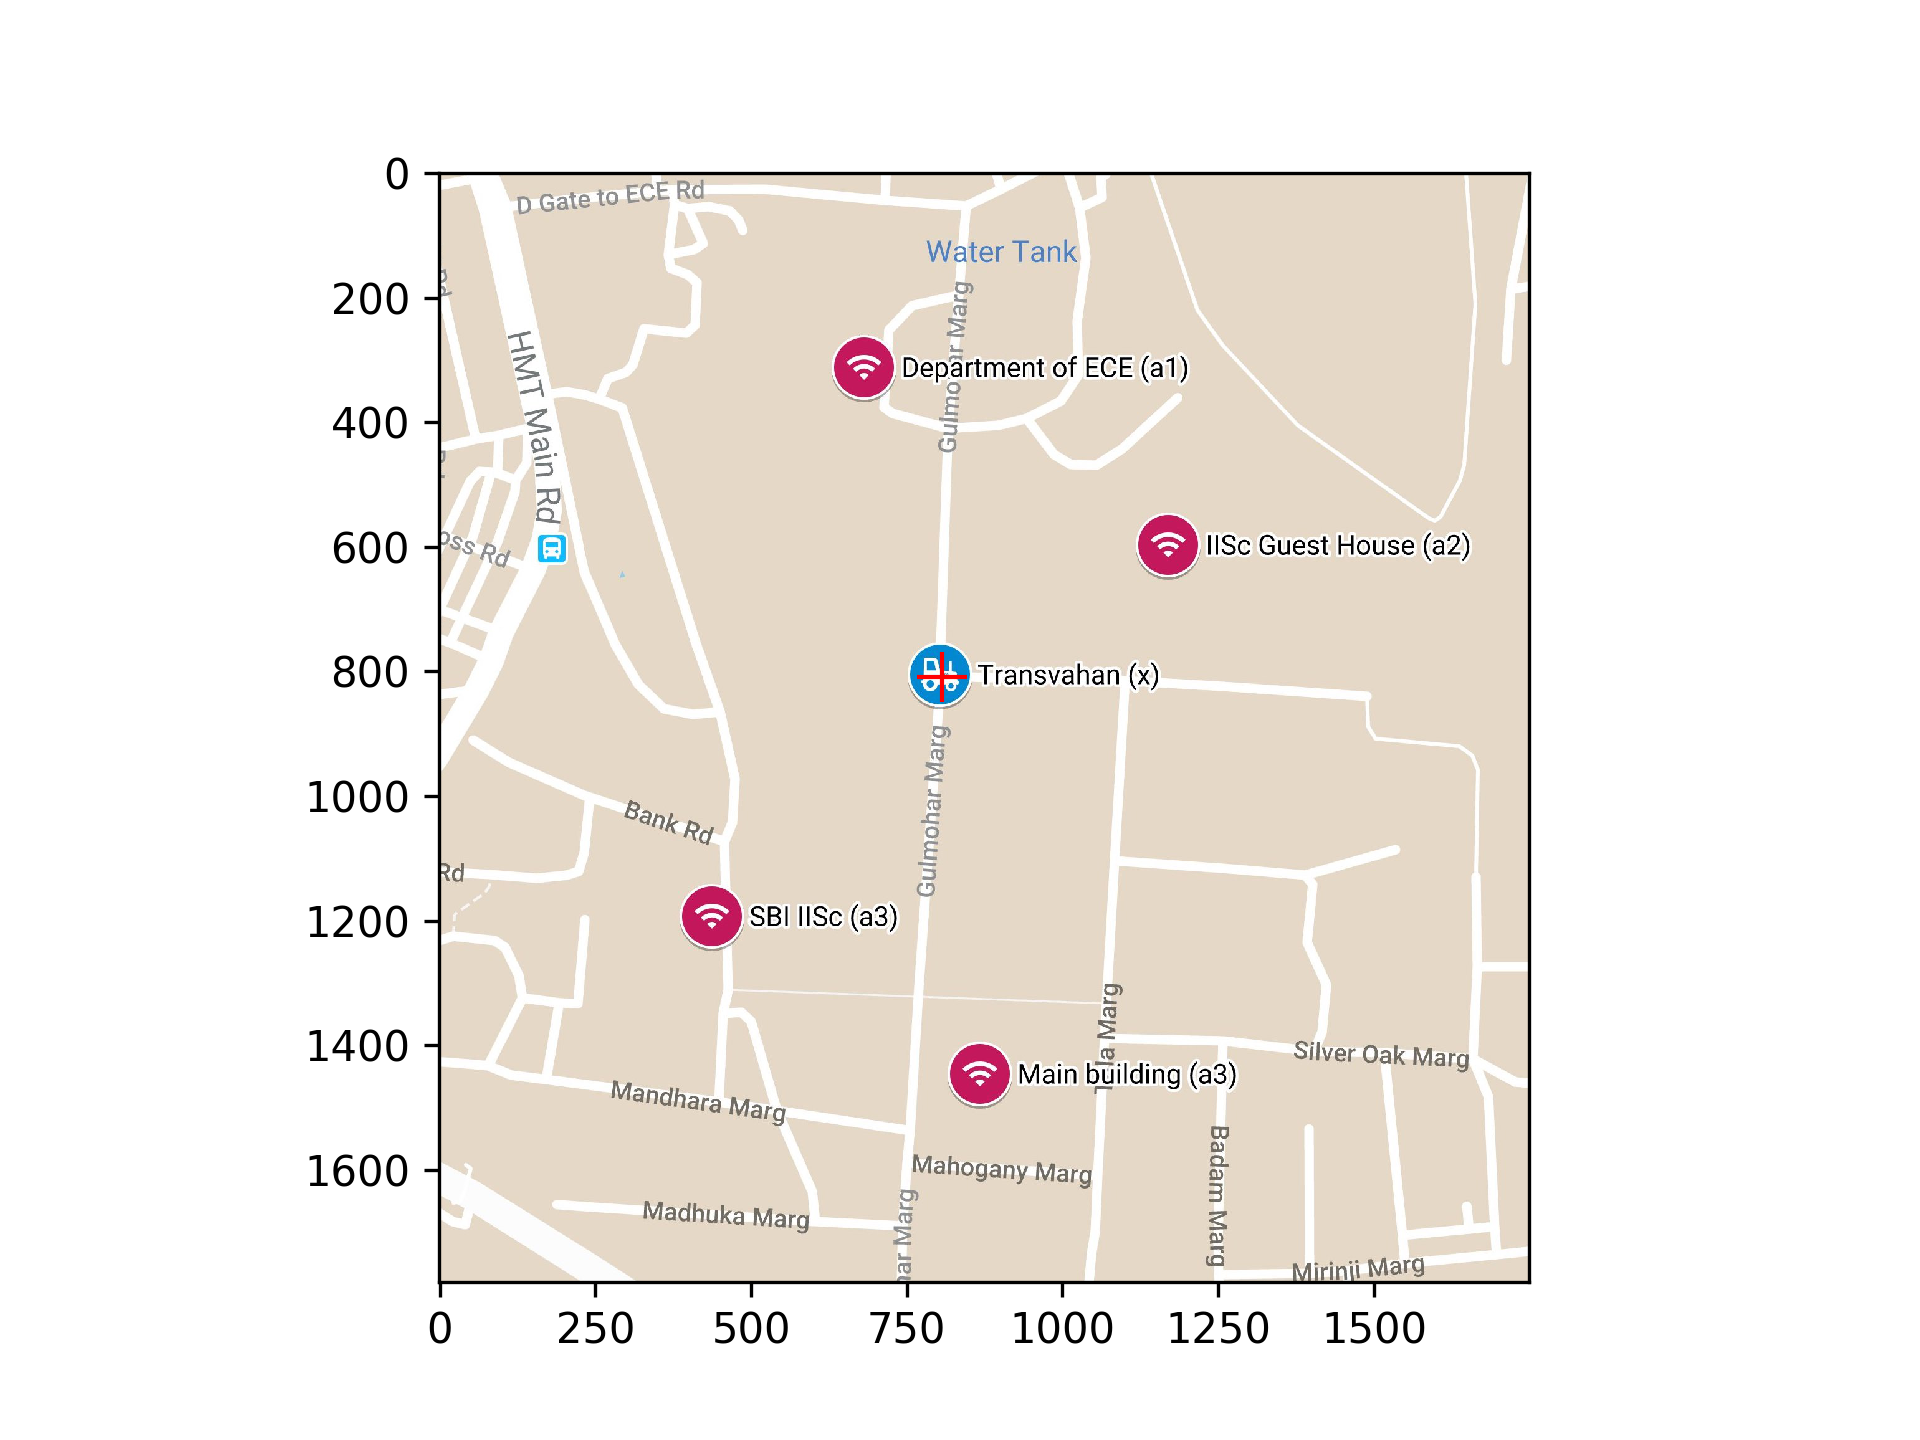
\includegraphics[width=\linewidth]{../results/MLE_map_loc.png}
	\caption{Estimated location of Transvahan using MLE}
	\label{fig:MLE}
\end{figure}





\newpage
\problem{B: Problem 2 Estimated location of the	Transvahan using BLUE estimator}

\vspace{6em}

\begin{figure}[h]
	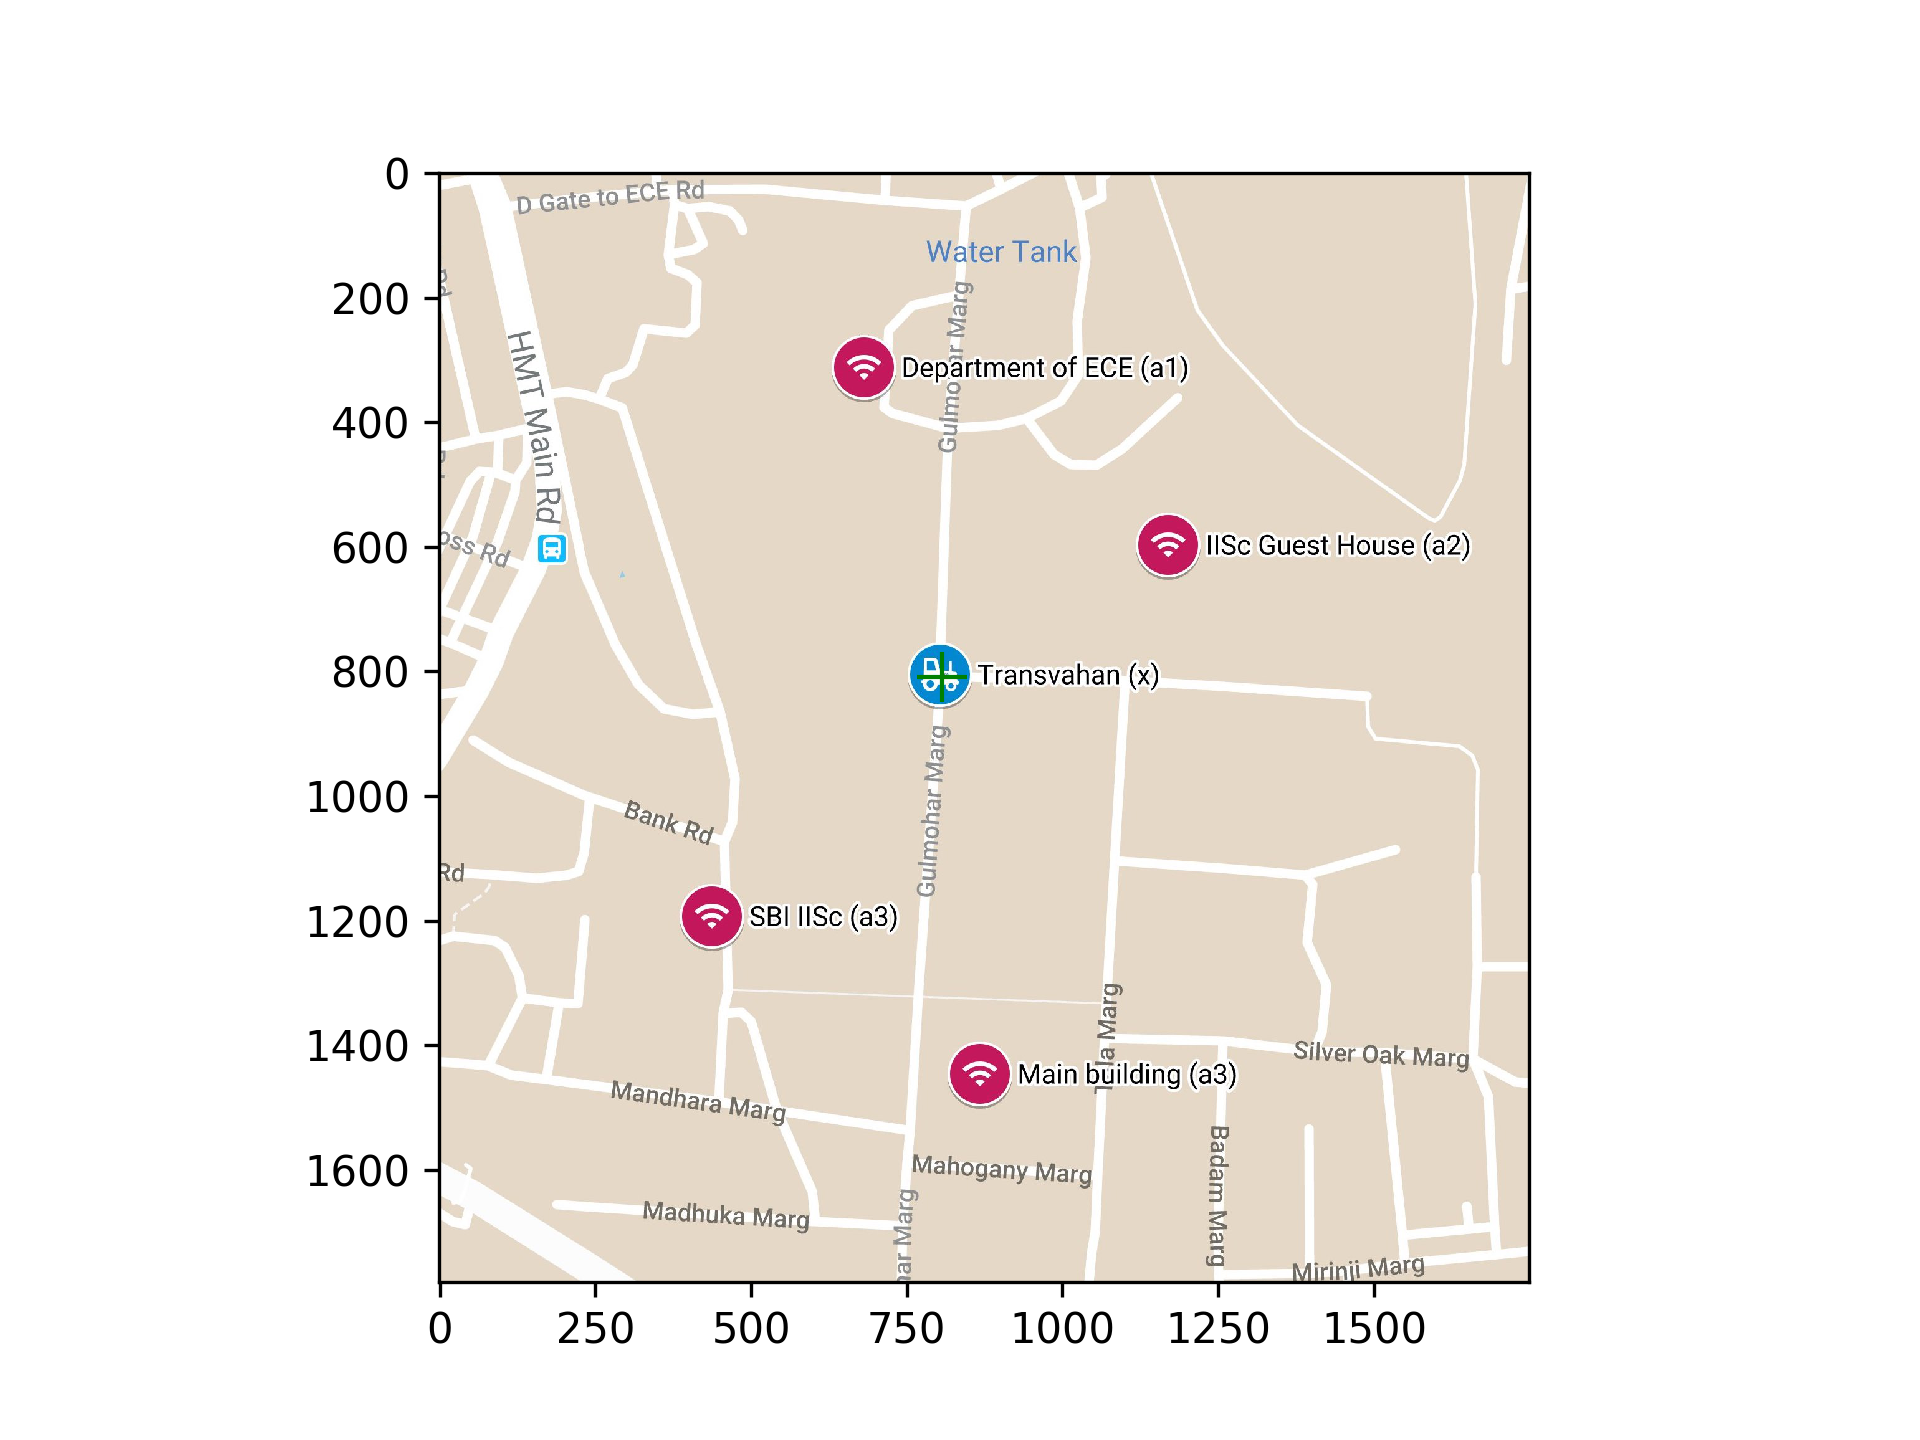
\includegraphics[width=\linewidth]{../results/BLUE_map_loc.png}
	\caption{Estimated location of Transvahan using MLE}
	\label{fig:BLUE}
\end{figure}




\newpage
\problem{B: Problem 3 Comparison of CRLB and mean squared error of MLE \& BLUE estimators}

\vspace{6em}

\begin{figure}[h]
	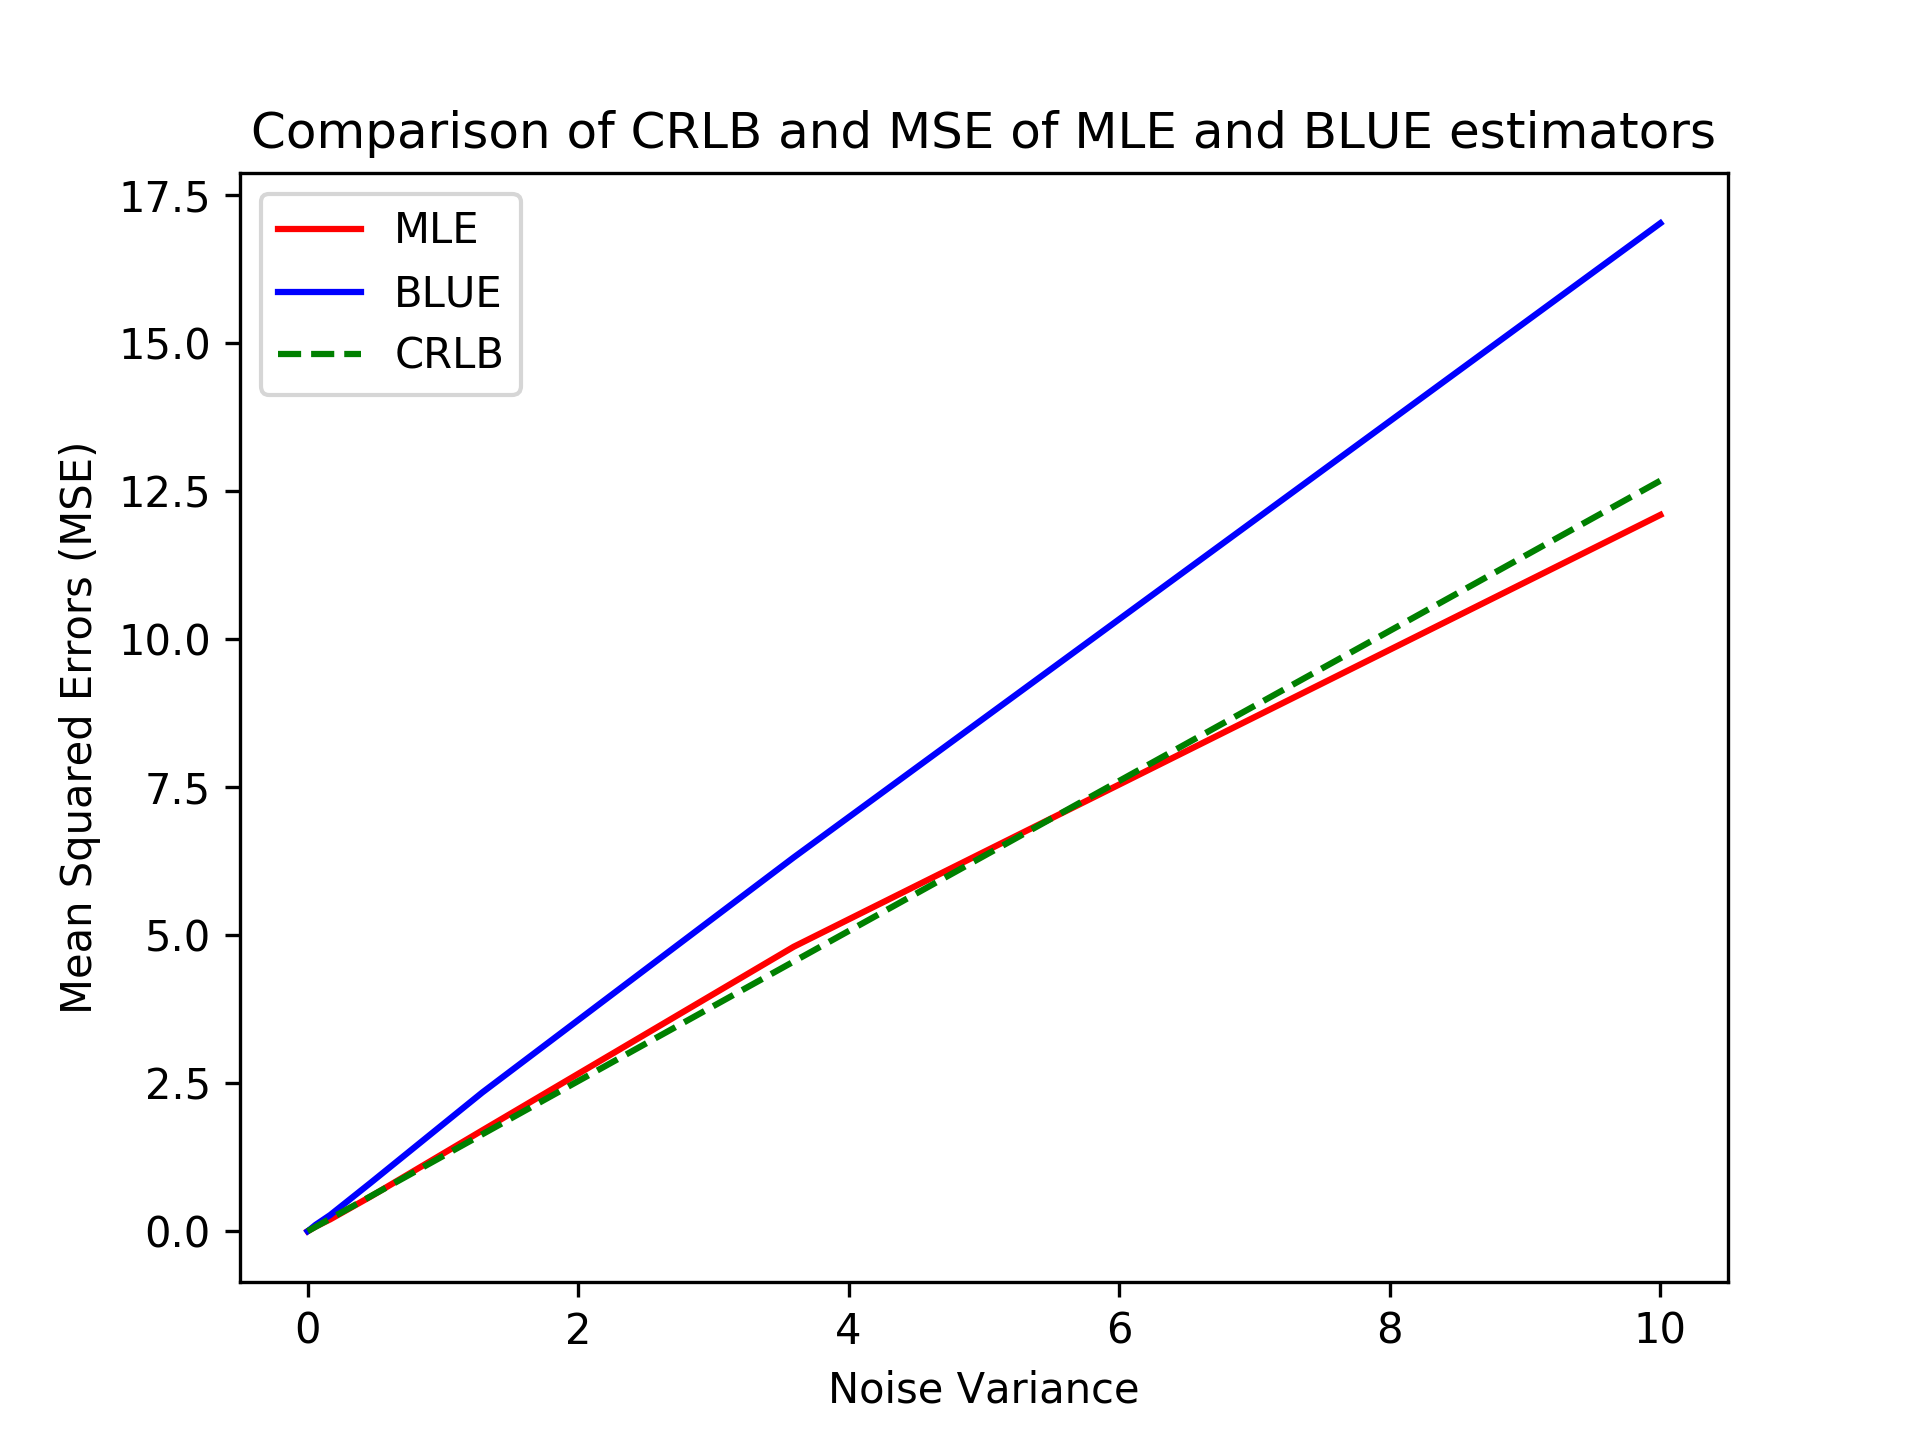
\includegraphics[width=\linewidth]{../results/MSE.png}
	\caption{Estimated location of Transvahan using MLE}
	\label{fig:MSE}
\end{figure}





\newpage
\problem{C: Appendices (Python codes)}
\solution The entire program is written in four python files - main.py, CRLB.py, MLE.py and BLUE.py. The codes are provided below and are also available at \url{https://github.com/vineeths96/TDOA-Localization} GitHub repository. (Repository access is private as of now. Access can me made available, if necessary).

\subproblem{main.py}
\inputminted[frame=lines, framesep=2mm, baselinestretch=1.2, fontsize=\footnotesize, linenos]{python}{../main.py}


\newpage
\subproblem{CRLB.py}
\inputminted[frame=lines, framesep=2mm, baselinestretch=1.2, fontsize=\footnotesize, linenos]{python}{../CRLB.py}


\newpage
\subproblem{MLE.py}
\inputminted[frame=lines, framesep=2mm, baselinestretch=1.2, fontsize=\footnotesize, linenos]{python}{../MLE.py}


\newpage
\subproblem{BLUE.py}
\inputminted[frame=lines, framesep=2mm, baselinestretch=1.2, fontsize=\footnotesize, linenos]{python}{../BLUE.py}


\end{document} 
